
$\because $ the points are collinear, we create a matrix
\begin{align}
  \vec{M} &=  \myvec{\vec{B}-\vec{A}&\vec{C}-\vec{A}}^{\top}
  \\
%\end{align}
%where $rank(\vec{M})=1$.We have the matrix $\vec{M}$ as,
%\begin{align}
    & = \myvec{1+5&p-1\\4+5&-2-1} \\
    & =   \myvec{6&p-1\\9&-3}
\end{align}
Now we row reduce the matrix $\vec{M}$,
\begin{align}
\myvec{6&p-1\\9&-3}
\xleftrightarrow{R_1\leftrightarrow R_2}
\myvec{9&-3\\6&p-1}
\\
\xleftrightarrow{R_1\rightarrow \frac{R_1}{3}}
\myvec{3&-1\\6&p-1}
\\
\xleftrightarrow{R_2\rightarrow R_2-2R_1}
\myvec{3&-1\\0&p+1}
\\
\xleftrightarrow{R_1\rightarrow \frac{R_1}{3}}
\myvec{1&\frac{-1}{3}\\0&p+1}
\end{align}
Since $rank(\vec{M})=1$,we have
\begin{align}
 p+1=0 \\
\implies p=-1
 \end{align}
 Fig. \ref{vec/2006/147Graphical solution}  verifies that the points are indeed collinear for $p = -1$.
 %  
\begin{figure}[ht]
    \centering
    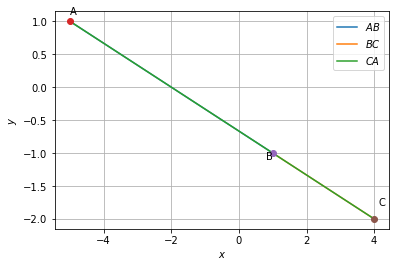
\includegraphics[width=\columnwidth]{vectors/solutions/2006/17/collinear.png}
    \caption{Collinear}
    \label{vec/2006/147Graphical solution}
\end{figure}

 


